\begin{SCfigure}
  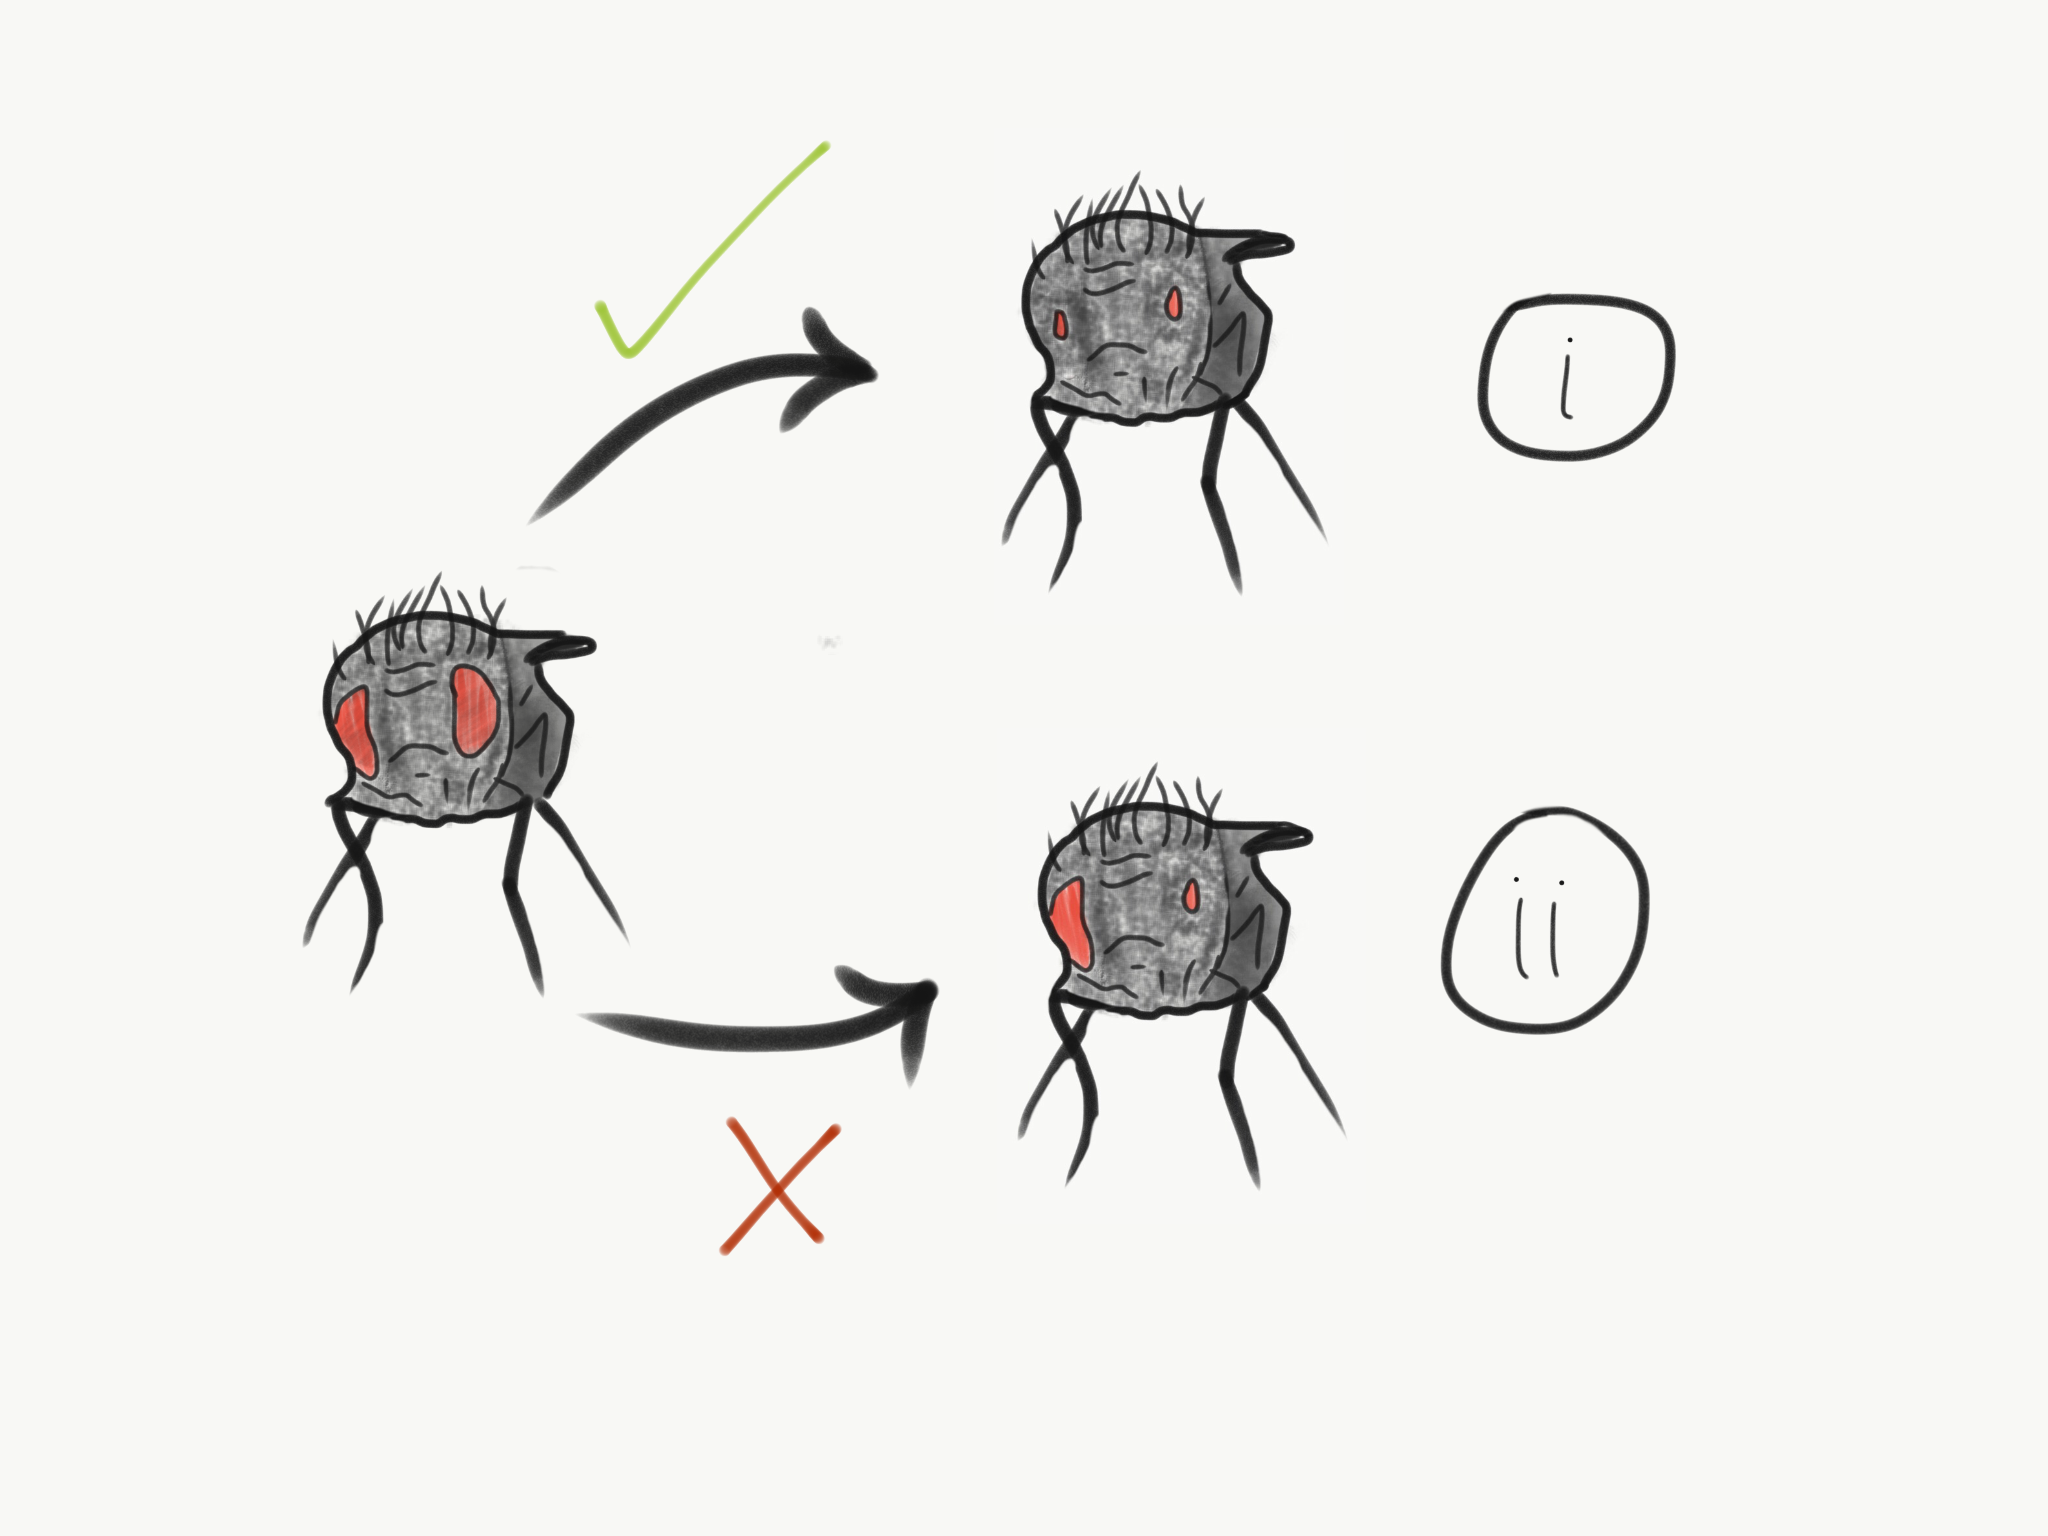
\includegraphics[width=0.5\textwidth]{img/canalization_example}
  %\captionsetup{singlelinecheck=off,justification=raggedright}
  \caption[Canalization in \textit{Drosophila melangoster} In Artificial Selection Experiments]{This cartoon depicts an artificial selection experiment on \textit{Drosophila melangoster}. In treatment i, selection is made for a bilaterally symmetric trait --- overall decreased eye size. Because this bilaterally symmetric trait can be produced through heritable variation, artificial selection succeeds. In treatment ii, artificial selection for a non-bilaterally symmetric trait --- relatively smaller right eye size --- fails because, due to the nature of the development process of \textit{Drosophila}, heritable variation that produces this trait is not readily possible.}
  \label{fig:canalization_example}
\end{SCfigure}
